\documentclass{spisok-article}

\title{О распараллеливании задачи численной проверки 
 частотного критерия отсутствия периодических режимов 
 для задачи управления в классе ортогональной системы  кусочно-постоянных функций}

\author{%
  Леонов Г. А.,
  д.ф.-м.н., профессор СПбГУ,

  Бурова И. Г.,
  д.ф.-м.н., профессор СПбГУ,

  Астахов М. О.,
  студент кафедры прикладной кибернетики СПбГУ
}

\begin{document}

\maketitle

\begin{abstract}
В настоящей работе рассматривается задача вычисления
определенных интегралов в задаче проверки частотного критерия, 
используются идеи по алгоритмической оптимизации, приводящие к уменьшению времени вычислений.
\end{abstract}

\section{Введение}

Задача поиска периодических решений систем управления является широко исследуемой в теории управления [1-5]. Для получения критерия отсутствия колебаний в нелинейной системе автоматического управления функциям входа и выхода ставится в соответствие ряды Фурье по ортогональной системе функций. В результате задача проверки критерия сводится к вычислению двойных интегралов. С помощью средств OpenMP  разрабатываются алгоритмы, позволяющие получить значительные преимущества по времени исполнения [6].
\section{Математическая постановка задачи}

Рассматривается система
\begin{equation}
\label{system1}
\left\{
\begin{array}{l}
\frac{dx}{dt} = Ax + b\varphi(\sigma),\\
\sigma = c^{*}x,\\
\end{array}
\right.
\mbox{ } \mbox{ } \mbox{ } \mbox{ } \mbox{ } x_{0} = x(0)
\end{equation}
где $A$ -- постоянная $n \times n$ -- матрица, $b$ и $c$ -- постоянные матрицы размерности $n \times m$ и $n \times l$ соответственно, $\varphi(\sigma)$ -- симметричная кусочно-непрерывная нелинейная функция. Операция $*$ означает транспонирование в вещественном случае [4].

Пусть, дополнительно, функция $\varphi(\sigma)$ удовлетворяет условию [1, 2]
\begin{equation}
\label{conditions1}
\begin{gathered}
0 \leq \frac{\varphi(\sigma)}{\sigma} \leq M  \mbox{   } \forall \sigma \neq 0,\\
\varphi(0)=0,
\end{gathered}
\end{equation}
где $M$ -- некоторое конечное число.

Следовательно, отсюда

\begin{equation}
\label{conditions3}
\varphi (\sigma - \frac{\varphi}{M}) \geq 0.
\end{equation}

Пусть теперь у системы~(\ref{system1}) существует периодическое решение частоты $\omega$, разлагающееся в почти всюду сходящийся обобщенный ряд Фурье по полной ортогональной системе функций $\{\varphi_{k}(t)\}_{k=1}^{\infty}$ в пространстве $L_2([a,b])$, так что функциям $\varphi(\sigma(t))$ и $\sigma(t)$ можно поставить в соответствие обобщенные ряды Фурье [7-9].

\begin{equation}
\label{equation1}
\varphi(\sigma) = \varphi(\sigma(t)) = \sum\limits^{\infty}_{k=0} {c_k\varphi_k(t)},
\end{equation}

Далее, для системы~(\ref{system1}) верно соотношение [1]:

\begin{equation}
\label{equation6}
\sigma(t) = \alpha(t) + \int\limits^{t}_{0} {\gamma(t-\tau)\varphi(\tau)d\tau},
\end{equation}
где $\alpha(t) = c^{*}e^{At}x_{0}$, $\gamma(t,\tau) = c^{*}e^{A(t-\tau)}b$ и $x_{0} = x(0).$

Откуда мы получаем разложение функции $\sigma(t)$ в следующем виде:

\begin{equation}
\label{equation8}
\sigma(t) = \sum\limits^{\infty}_{k=0} {c_k\left(\sum\limits^{\infty}_{n=0} {a_{kn}\varphi_{n}(t)}\right)} = \sum\limits^{\infty}_{n=0} {\left( \sum\limits^{\infty}_{k=0} { c_{k}a_{kn} } \right)\varphi_{n}(t)},
\end{equation}
где $a_{kn} = \int\limits_a^b \left( \int\limits_0^s \gamma(s-\tau){\varphi}_k(\tau)\,d\tau\right){\varphi}_n(s)\,ds$.

Подставим полученные разложения~(\ref{equation8}), ~(\ref{equation1}) в секторное условие~(\ref{conditions3}) и проинтегрируем по периоду $[a,b]$,  имеем:

\begin{equation}
\label{equation9}
{\sum\limits^{\infty}_{i=-\infty}c_i\left({\sum\limits^{\infty}_{k=-\infty} c_k a_{ki} - \frac{c_i}{M}}\right)} \geq 0.
\end{equation}

Полученное выражение~(\ref{equation9}) есть квадратичная форма относительно $c_i$.

Периодический режим системы может существовать тогда и только тогда, когда выполнено неравенство~(\ref{equation9}).

Сформулируем критерий Сильвестра [10]: для отрицательной определённости квадратичной формы необходимо и достаточно, чтобы угловые миноры чётного порядка её матрицы были положительны, а нечётного порядка -- отрицательны.

Тогда можно сформулировать критерий неколебательности: если квадратичная форма отрицательно определена по критерию Сильвестра, то система не имеет периодических режимов частоты $\omega$ .

\section{Программная реализация}

Алгоритм был реализован на компьютере со следующими характеристиками:

Процессор: восьмиядерный процессор Intel Core i7-4700HQ (2.40GHz), Память: 8 Gb, Операционная система: Windows 8.1, Среда разработки: Microsoft Visual Studio 2013

Далее численно проверяется полученный критерий для разных ортонормированных систем функций и передаточных функций W(p).

Цель: Найти ортогональную систему функций, для которой получим большее M в условии на сектор $ 0 \leq \frac{\varphi(\sigma)}{\sigma} \leq M $ по сравнению с другими системами.

Для численного эксперимента решалась следующая задача: необходимо оптимизировать вычисление элементов матрицы квадратичной формы. В процессе вычислений необходимо распараллелить выполнение двойного цикла.

На языке $C^{++}$ были реализованы последовательный и параллельный алгоритмы для численной проверки критерия неколебательности, полученного
в предыдущем разделе.
\bigskip

Алгоритм:
\begin{itemize}
\item
Определение начальных параметров: частота $\omega$, количество чле-
нов разложения $N$, определить матрицы $A$, $b$, $c$;

\item
построение системы разложения;

\item
построение промежуточной системы -- переразложение по ортонормированной системе;

\item
вычисление коэффициентов матрицы квадратичной формы, используя двойной цикл;

\item
вычисление определителей для установления области неколебательности.
\end{itemize}

Для распараллеливания вычислений используются средства
OpenMP. В OpenMP есть специальные средства для распараллеливания
цикла.

%\lstset{language=C++,basicstyle=\footnotesize}
\begin{verbatim}
#pragma omp parallel reduction (+: S)
    {
        #pragma omp for
        for (int i = 1; i < N; i += 1)
        {
            for (int j = 1; j < N; j += 1)
            {
                A_ji = int(midfunc[j]*sin_array[i]/T;
            }

        }
\end{verbatim}

Директива $parallel$ определяет параллельную область, границы которой определяется фигурными скобками. Для вычисления матрицы, элементами
которой являются интегралы будем использовать вложенные циклы.
Выше представлен один из циклов.

Время работы функции вычисления интегралов  при распараллеливании вычислений значительно меньше времени вычисления  при последовательной реализации. Кроме того, время вычислений несколько меняется при каждом новом  запуске программы.  Программа выполняет некоторое наперед заданное число экспериментов и на выходе выдает значение интеграла и три величины:     среднее, минимальное и максимальное время работы, как показано на Рис.~\ref{ris1:image} и Рис.~\ref{ris2:image}.

\begin{figure}[h]
	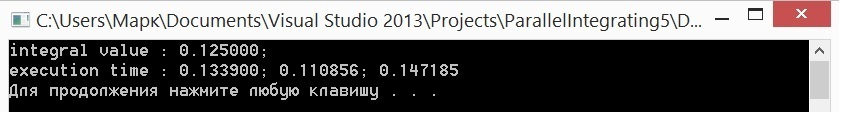
\includegraphics[width=1\linewidth]{paral1.jpg}
	\caption{Результат работы последовательной версии программы}
	\label{ris1:image}
\end{figure}

\begin{figure}[h]
	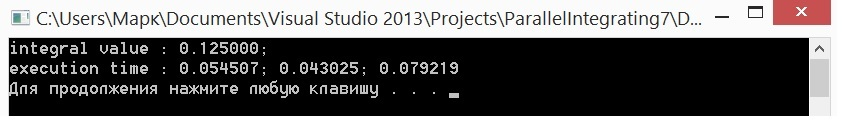
\includegraphics[width=1\linewidth]{paral2.jpg}
	\caption{Результат работы параллельной версии программы}
	\label{ris2:image}
\end{figure}

Рассмотрим некоторые сравнительные характеристики для последовательной и параллельной версии программ.


На Рис.~\ref{ris3:image} изображен график, показывающий зависимость между количеством слагаемых частичной суммы ряда Фурье $N$ и ускорением, которое равно отношению среднего времени работы последовательной программы к параллельной.

\begin{figure}[h]
\begin{center}
	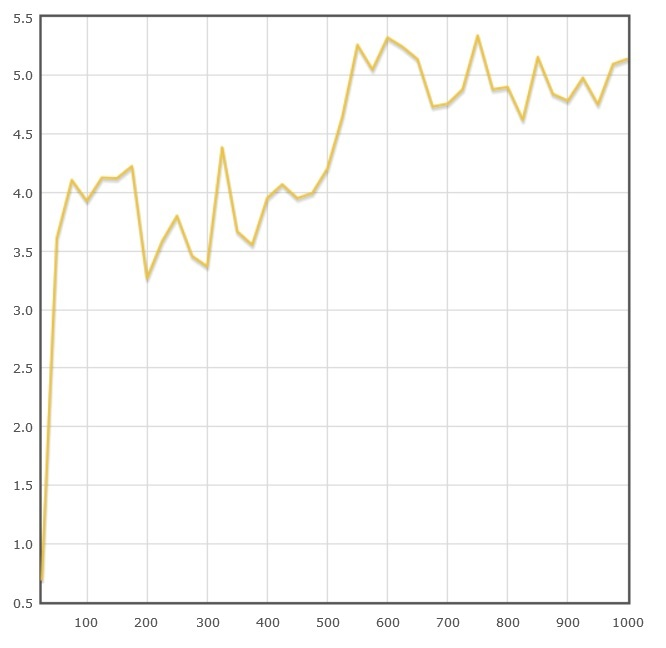
\includegraphics[width=81mm]{paral3.jpg}
	\caption{График зависимости ускорения от количества слагаемых частичной суммы ряда Фурье $N$ для 4-х потоков}
	\label{ris3:image}
\end{center}
\end{figure}

Ниже представлена таблица ускорений для разного количества потоков: 2, 4, 8 в зависимости от количества слагаемых частичной суммы ряда Фурье $N$.
\bigskip
\begin{center}
\begin{tabular}{|c|c|c|c|c|c|c|c|c|c|}
\hline
 &N = 8 & N = 16 & N = 32 & N = 64 & N = 128 & N = 256 & N = 512 \\
\hline
2 & 0.87500 & 1.05455 & 1.21071 & 1.41031 & 1.50764 & 1.64587 & 1.69363 \\
\hline
4 & 0.769231 & 1.79412 & 2.50435 & 3.09677 & 3.048 & 3.47957 & 3.50836 \\
\hline
8 & 0.846154 & 2.21053 & 3.09836 & 3.68644 & 3.73731 & 4.44577 & 5.32119 \\
\hline
\end{tabular}
\end{center}
\bigskip

\section{Заключение}

В работе исследовалась задача вычисления двойных интегралов для численной проверки частотного критерия для системы управления, рассмотрен алгоритм, позволяющий численно проверить критерий неколебательности. Далее были изложены идеи по уменьшению времени вычислений путем распараллеливания процессов. На основе алгоритма были реализованы последовательная и параллельная версии программы. В результате  удалось добиться ускорения процесса вычисления в несколько раз.

\renewcommand \refname{Литература}
\begin{thebibliography}{8}

\bibitem{a} Леонов Г.А. О проблеме Айзермана // Автоматика и телемеханика.  2009, № 7. 
 С. 37-49.
\bibitem{b} Айзерман М.А. Об одной проблеме, касающейся устойчивости "в большом" динамических систем // Успехи математических наук.
- 1949.  Т. 4, № 4.  C. 187-188.
\bibitem{c} Леонов Г.А. О необходимости частотного условия абсолютной устойчивости стационарных систем в критическом случае пары чисто мнимых корней // Докл. АН СССР.  1970. 
     Vol. 193.
\bibitem{d} Леонов Г.A. Теория управления.  СПб.: Изд-во C.-Петерб. ун-та, 2006.  233 c.
\bibitem{e} Гарбер Е.Д. О частотных критериях отсутствия периодических режимов, Автомат. и телемех., 1967, № 11, c.178-182.
\bibitem{f} Антонов А.С. Параллельное программирование с использованием технологии OpenMP: Учебное пособие. - Москва.: Изд-во МГУ, 2009.  77 с.
\bibitem{g} Крылов В.И. Приближенное вычисление интегралов. - Москва.: Изд-во Наука, 1967.  500~c.
\bibitem{h} Голубов Б. И., Ефимов А. В., Скворцов В. А. Ряды и преобразования Уолша: теория и применения. - М.: Изд-во Наука, 1987.  344~с.

\bibitem{i} Зигмунд А. Тригонометрические ряды. T.1,2. М.: Мир, 1965.

\bibitem{j} Беклемишев Д.В. Курс аналитической геометрии и линейной алгебры. - М.: Наука, 1971. - 328~с.

\end{thebibliography}

\end{document}
